\documentclass{article}
\usepackage{graphicx} % Required for inserting images
\usepackage[utf8]{inputenc}
\usepackage{amsmath,amsfonts,amssymb,amsthm}
\usepackage{enumerate,bbm}
\usepackage{tikz,tikz-cd, graphicx,color,mathrsfs,color,hyperref,boldline}
\usepackage{caption,float}
\usepackage[a4paper,margin=1in,footskip=0.25in]{geometry}

\usepackage{listings}
\usepackage{xcolor}

\usepackage{tabularx,capt-of}

\usepackage{blindtext}
%Image-related packages
\usepackage{graphicx}
\usepackage{subcaption}
\usepackage[export]{adjustbox}
\usepackage{lipsum}

%hyperref setup
\hypersetup{
    colorlinks=true,
    linkcolor=blue,
    filecolor=magenta,      
    urlcolor=cyan,
    pdftitle={Overleaf Example},
    pdfpagemode=FullScreen,
    }

%New colors defined below
\definecolor{codegreen}{rgb}{0,0.6,0}
\definecolor{codegray}{rgb}{0.5,0.5,0.5}
\definecolor{codepurple}{rgb}{0.58,0,0.82}
\definecolor{backcolour}{rgb}{0.95,0.95,0.92}

%Code listing style named "mystyle"
\lstdefinestyle{mystyle}{
  backgroundcolor=\color{backcolour}, commentstyle=\color{codegreen},
  keywordstyle=\color{magenta},
  numberstyle=\tiny\color{codegray},
  stringstyle=\color{codepurple},
  basicstyle=\ttfamily\footnotesize,
  breakatwhitespace=false,         
  breaklines=true,                 
  captionpos=b,                    
  keepspaces=true,                 
  numbers=left,                    
  numbersep=5pt,                  
  showspaces=false,                
  showstringspaces=false,
  showtabs=false,                  
  tabsize=2
}

%"mystyle" code listing set
\lstset{style=mystyle}

\theoremstyle{definition}
\newtheorem{defn}{Definition}[section]
\newtheorem{example}[defn]{Example}
\theoremstyle{remark}
\newtheorem{rem}{Remark}
\newtheorem{remS}[section]{defn}

\theoremstyle{plain}
\newtheorem{lem}[defn]{Lemma}
\newtheorem{thm}[defn]{Theorem}
\newtheorem{prop}[defn]{Proposition}
\newtheorem{fact}[defn]{Fact}
\newtheorem{crly}[defn]{Corollary}
\newtheorem{conj}[defn]{Conjecture}

%\newtheorem*{programming*}{Programming Task}

%\newtheorem{innercustomgeneric}{\customgenericname}
%\providecommand{\customgenericname}{}
%\newcommand{\newcustomtheorem}[2]{%
%  \newenvironment{#1}[1]
%  {%
%   \renewcommand\customgenericname{#2}%
%   \renewcommand\theinnercustomgeneric{##1}%
%   \innercustomgeneric
%  }
%  {\endinnercustomgeneric}
%}

%\newcustomtheorem{question}{Question}
%\newcustomtheorem{programming}{Programming Task}

\newcommand{\NN}{\mathbb{N}}
\newcommand{\ZZ}{\mathbb{Z}}
\newcommand{\QQ}{\mathbb{Q}}
\newcommand{\RR}{\mathbb{R}}
\newcommand{\CC}{\mathbb{C}}
\newcommand{\PP}{\mathbb{P}}
\newcommand{\FF}{\mathbb{F}}

\newcommand{\calD}{\mathcal{D}}

\newcommand{\id}{\operatorname{id}}
\newcommand{\Hom}{\operatorname{Hom}}

\newcommand{\sol}{\textit{Solution: }}
\newcommand{\Res}{\operatorname{Res}}

\title{II Algebraic Topology}
\author{Kevin}
\date{October 2024}

\begin{document}
\maketitle
\section{Background and Conventions}
\begin{lem}[Gluing lemma]
    Let $X,Y$ be topological spaces, $f:X\to Y$ a function, If $X=C_1\cup C_2$ for some closed sets $C_1,C_2$, then $f$ is continuous if and only if $f|_{C_i}$ is continuous
\end{lem}
\begin{thm}[Lebesgue number lemma]
Let $(X,d)$ be a compact metric space. For every open cover $\{U_\alpha\}_{\alpha\in I}$ of $X$, there exists $\delta>0$ s.t. each open ball $B_\delta(x)$ is contained entirely in some $U_\alpha$.    
\end{thm}
\begin{defn}[Finite cell complex]
A finite cell complex (CX) is a space $X$ obtained by
\begin{enumerate}
    \item Start a finite set $X^0$ with the discrete topology, called the $0$-skeleton.
    \item Inductively, the $n$-skeleton $X^n$ is obtained from $X^{n-1}$ by attaching finitely $n$-cells
    \item Stop after finitely many steps, so $X=X^k$ for some $k$ which is defined as the dimension of $X$.
\end{enumerate}
\end{defn}

\section{Homotopy and the Fundamental Group}
\subsection{Homotopy}
\begin{defn}[Homotopy]
    Two maps $f,g:X\to Y$ are homotopic if there exists a map $H:X\times I\to Y$ s.t. $H|_{X\times{0}}=f$ and $H|_{X\times\{1\}}=g$. We write $f\simeq_H g$. If $A\subseteq X$ is a subset, then we say that $f\simeq_H g$ rel $A$ if in addition $\forall t\in I,\ \forall a\in A,\ H(a,t)=f(a)=g(a)$.
\end{defn}
\begin{prop}
    ``$\simeq$ rel $A$'' on $\Hom_{\mathbf{Top}}(X,Y)$ is an equivalence relation.
\end{prop}
\begin{proof}
    Trivial. Just compute.
\end{proof}
\begin{defn}[Homotopy Equivalence]
    Say a map $f:X\to Y$ is a homotopy equivalence if there exists $g:Y\to X$ s.t. $fg\simeq \id_Y$ and $gf\simeq id_X$. In this situation we say that $X\simeq Y$ ($X$ is homotopy equivalent to $Y$.)
\end{defn}
\begin{defn}
    $X$ is contractible if $X$ is htpy equiv. to a singleton.
\end{defn}
\begin{lem}
    If $f_0,f_1:X\to Y$, $g_0,g_1:Y\to Z$ are maps s.t. $f_0\simeq_H f_1$ and $g_0\simeq_G g_1$, then $g_0f_0\simeq g_1f_1$.
\end{lem}
\begin{proof}
    Observe $g_0f_0\simeq_{g_0H}g_0f_1\simeq_{G\circ(f_1\times\id_I))}g_1f_1$.
\end{proof}
\begin{prop}
    Homotopy equivalence is an equiv. rel. on top. spaces.
\end{prop}
\begin{defn}
    $X$ a top. space, and $A\subseteq X$ a subspace. A deformation retraction from $X$ to $A$ is a map $r:X\to A$ s.t. $r\circ i=\id_A$ and $i\circ r\simeq \id_X$. If the homotopy is rel $A$ then we say that this is a strong deformation retraction.
\end{defn}
\subsection{Paths}
\begin{itemize}
    \item \textbf{Notation}: a path $\gamma:I\to X$ from $x_0$ to $x_1$ is denoted $\gamma:x_0\rightsquigarrow x_1$.
    \item \textbf{Concatenation}: If $\gamma:x_0\rightsquigarrow x_1$ and $\gamma':x_1\rightsquigarrow x_2$, then $\gamma\cdot\gamma':x_0\rightsquigarrow x_2$ is defined in the obvious way, i.e., traverse through $\gamma$ at double the original speed and then traverse through $\gamma'$ at double the speed. One can easily figure out an explicit formula in terms of $\gamma$ and $\gamma'$.
    \item \textbf{Inverse}: $\gamma^{-1}(t)=\gamma(1-t)$;
    \item \textbf{Constant path}: $c_{x_0}$ is the trivial path from $x_0$ to itself.
    \item \textbf{The set of path components:} $\pi_0(X)$.
\end{itemize}
\begin{prop}
    $\pi_0$ is a (covariant) functor $\pi_0:\mathbf{Top}\to \mathbf{Set}$. In fact, $\pi_0$ factors through $\mathbf{HoTop}$.
\end{prop}
\begin{defn}
    Two paths $\gamma,\gamma':x_0\rightsquigarrow x_1$ are path-homotopic if $\gamma\simeq\gamma'$ rel $\partial I$.
\end{defn}
\begin{lem}
    If $\gamma_0,\gamma_1:x_0\rightsquigarrow$ are path-homotopic and $\gamma_0',\gamma_1':x_1\rightsquigarrow x_2$ are also path-homotopic, then $\gamma_0\cdot\gamma_0'$ and $\gamma_1\cdot\gamma_1'$ are path-homotopic.
\end{lem}
\begin{proof}
    c.f. lemma 2.5.
\end{proof}
\begin{prop}
    Path concatenation has the following properties.  Suppose $\gamma_i:x_i\rightsquigarrow x_{i+1}$ for $i=0,1,2$. Then,
    \begin{enumerate}
        \item $(\gamma_0\cdot\gamma_1)\cdot\gamma_2\simeq\gamma_0\cdot(\gamma_1\cdot\gamma_2)$ rel $\partial I$.
        \item $c_{x_0}\cdot\gamma_0\simeq \gamma_0$ rel $\partial I$ and $\gamma_0\cdot c_{x_1}\simeq \gamma_0$ rel $\partial I$.
        \item $\gamma_0\cdot\gamma_0^{-1}\simeq c_{x_0}$ rel $\partial I$, $\gamma_0^{-1}\cdot\gamma_0\simeq c_{x_1}$ rel $\partial I$.
    \end{enumerate}
\end{prop}
\begin{proof}
    Not hard, will include later.
\end{proof}
The above proposition gives us an object called the fundamental groupoid. [A category in which objects are points of the space and morphisms between objects are given by the set of homotopy classes of paths. Obviously every morphism is invertible.]

\subsection{The Fundamental Groups}
\begin{defn}
    Let $(X,x_0)$ be a pointed topological space. We define the its fundamental group of $X$ based at $x_0$, denoted $\pi_1(X)$, as the group of homotopy classes of loops, i.e., $[(I,\partial I),(X,x_0)]$.
\end{defn}
It is indeed a group. The group operation is given by concatenation of loops. Alternatively, one can also define the fundamental group $\pi_1(X,x_0)$ as the group $[(S^1,\ast),(X,x_0)]$.
\begin{prop}
    $\pi_1$ is a functor $\mathbf{Top}_\ast\to\mathbf{Grp}$ which factors through $\mathbf{HoTop}_\ast$.
\end{prop}
\begin{proof}
    Just need to check a few things.\begin{enumerate}
        \item Check that the induced map is indeed a well-defined homomorphism.
        \item If two maps are based homotopic, then they induce the same hom on $\pi_1$.
        \item $\pi_1(\id_X)=\id_{\pi_1(X,x_0)}$;
        \item Functoriality
    \end{enumerate}
\end{proof}
\begin{prop}
    If $u:x_0\rightsquigarrow x_1$ is a path in $X$, then it induces a group isomorphism $u_\#:\pi_1(X,x_0)\to\pi_1(X,x_1)$ given by conjugating each loop by the path. This group iso has the following properties
    \begin{enumerate}
        \item If $u\simeq u'$ as paths, then $u_\#=u'_\#$.
        \item $(c_{x_0})_\#=\id_{\pi(X,x_0)}$.
        \item If $v:x_1\rightsquigarrow x_2$ then $(u\cdot v)_\#=v_\#\circ u_\#$.
        \item If $f:X\to Y$ is a map w/ $f(x_0)=y_0$, $f(x_1)=y_1$, then the following diagram commutes.
        \begin{center}
            % https://tikzcd.yichuanshen.de/#N4Igdg9gJgpgziAXAbVABwnAlgFyxMJZABgBpiBdUkANwEMAbAVxiRAB120sB9ARgAUADVIAPHsQCUIAL6l0mXPkIo+5KrUYs2nbvwEBNUgE8J0uQux4CRMnw31mrRBy69BI8X3PyQGK8pEavbUjtouuu6GJvzmGjBQAObwRKAAZgBOEAC2SGQgOBBIappObGk8nHRwOCDUDHQARjAMAAqK1iogDDBptRYgmTl51IVIAEyhWs4gTJXsAMR13U0t7QE2Lj19sr5DuYglY4gAzFNlLgJpnADGWBk3AARMkvPVtfWrbR2BW739eyyB0mBSKp3O4UGbxqywazW+Gy6236FBkQA
\begin{tikzcd}
{\pi_1(X,x_0)} \arrow[r, "f_\ast"] \arrow[d, "u_\#"] & {\pi_1(Y,y_0)} \arrow[d, "(f\circ u)_\ast"] \\
{\pi_1(X,x_1)} \arrow[r, "f_\ast"]                   & {\pi_1(Y,y_1)}                             
\end{tikzcd}
        \end{center}
    \end{enumerate}
\end{prop}
\begin{proof}
    $1)$-$3)$ are trivial. $4)$ follows from a direct computation.
\end{proof}
\begin{lem}
    Let $f,g:X\to Y$ be maps s.t. $f\simeq_H g$. Let $u=H(x_0,-)$. Then, the following diagram commutes.
    \begin{center}
        % https://tikzcd.yichuanshen.de/#N4Igdg9gJgpgziAXAbVABwnAlgFyxMJZABgBpiBdUkANwEMAbAVxiRAB120sB9ARgAUADVIAPHsQCUIAL6l0mXPkIo+5KrUYs2nbvwEBNUgDMB4qdLkLseAkTV8N9Zq0QcuvQUYDmZiZMsNGChveCJQYwAnCABbJDIQHAgkNU0XNmMeTjo4HFl5ECjYlOokpAAmamdtNyYs9gBifIjouMQEssRKtJqQb3qcvJkKGSA
\begin{tikzcd}
{\pi_1(X,x_0)} \arrow[r, "f_\ast"] \arrow[rd, "g_\ast"] & {\pi_1(Y,f(x_0))} \arrow[d, "u_\#"] \\
                                                        & {\pi_1(Y,g(x_0))}                  
\end{tikzcd}
    \end{center}
\end{lem}
\begin{proof}
The idea of the proof is the homotopy given by the following diagram. Take a loop $\gamma:I\to X$, then the homotopy $H$ and a deformation retraction $I\times I\to I\times\{0\}\cup\partial I\times I$ allows one to fill in the square and construct a homotopy $g\circ\gamma\simeq u^{-1}\cdot(f\circ\gamma)\cdot u$.
    \begin{figure}[H]
        \centering
        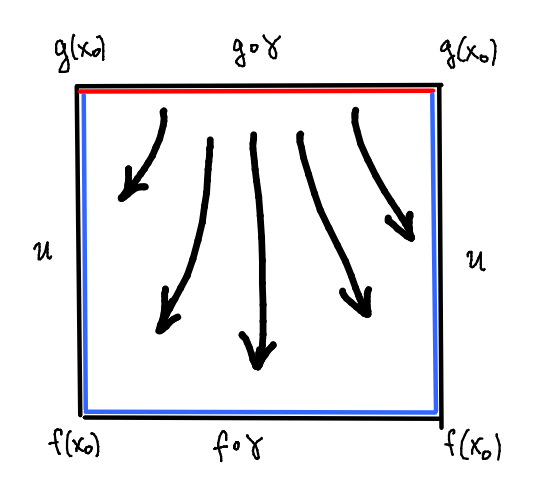
\includegraphics[width=0.5\linewidth]{Mich/pictures/algtop-lemma2.15.PNG}
    \end{figure}
\end{proof}
One can be more explicit and write down a formula for the homotopy.
\begin{defn}
    $X$ is simply connected if it is path-connected and $\pi_1(X,x_0)$ is trivial.
\end{defn}
\begin{lem}
    $X$ is simply connected $\Leftrightarrow$ for each pair $x_0,x_1\in X$, there is a unique homotopy class of paths between them.
\end{lem}
\begin{proof}
    ``$\Rightarrow$'': Path-connectedness implies the existence of such class. Trivial $\pi_1$ (the base point does not matter due to path-connectedness) implies that any two paths $\gamma,\mu:x_0\rightsquigarrow x_1$ are path homotopic as $[\gamma\cdot\mu^{-1}]=[c_{x_0}]$.

    ``$\Leftarrow$'': Existence of such homotopy class implies pathconnectedness. By uniqueness, given any loop, we can break it up into the concatenation of two paths then use the unique path homotopy class to deduce that the loop must be homotopically trivial.
\end{proof}

\section{Covering Spaces}
\subsection{Definition and Basic Properties}
\begin{defn}
    A space $\Tilde{X}$ is a covering space of $X$ with covering map $p:\Tilde{X}\to X$ if $\forall x\in X$, there exists an open nbd $U$ of $x$ s.t. $p^{-1}(U)=\bigsqcup_{\alpha\in A} V_\alpha$ for open subsets $V_\alpha\subseteq \Tilde{X}$ and $p|_{V_\alpha}:V_\alpha\to U$ is a homeo. (In this case we say that $U$ is evenly covered.)
\end{defn}
\begin{defn}
    Let $f:Y\to X$ be a map. A lift of $f$ along $p:\Tilde{X}\to X$ is a solution to the following problem.
    \begin{center}
        % https://tikzcd.yichuanshen.de/#N4Igdg9gJgpgziAXAbVABwnAlgFyxMJZABgBoBGAXVJADcBDAGwFcYkQBNEAX1PU1z5CKcqWLU6TVuwA6MvI1gACABo8+IDNjwEioqjQYs2iEGu4SYUAObwioAGYAnCAFskokDghIATIakTTXVHF3dEMi8fRH9JY3YHEJBnNyRI7w8aRiwwIKh6OAALKxAA+NM5BWVEi24gA
\begin{tikzcd}
                                                & \tilde X \arrow[d, "p"] \\
Y \arrow[r, "f"] \arrow[ru, "\tilde f", dashed] & X                      
\end{tikzcd}
    \end{center}
    i.e., if there exists $\tilde f:X\to \tilde X$ s.t. the above diagram commutes.
\end{defn}
\begin{lem}
    Let $p:\tilde X\to X$ be a covering map. Suppose we have two solutions to the lifting problem, i.e, there exists $\tilde f_0,\tilde f_1:Y\to\tilde X$ s.t. the following diagram commutes
    \begin{center}
        % https://tikzcd.yichuanshen.de/#N4Igdg9gJgpgziAXAbVABwnAlgFyxMJZABgBoBGAXVJADcBDAGwFcYkQBNEAX1PU1z5CKcqWLU6TVuwA6MvI1gACABo8+IDNjwEioqjQYs2iEGu4SYUAObwioAGYAnCAFskokDghIATIakTTXVHF3dEMi8fRH9JY3YHEBpGegAjGEYABQEdYRAnLGsACxwQkGc3JEjvD2SsMCC4CEYsKCS46VM5BWUHAH1idvSwNsQAZmJeUMqImhrETxT0rJyhdgLi0oD4rvksRRglfvIeSm4gA
\begin{tikzcd}
                                                                                & \tilde X \arrow[d, "p"] \\
Y \arrow[r, "f"'] \arrow[ru, "\tilde f_0", bend left] \arrow[ru, "\tilde f_1"'] & X                      
\end{tikzcd}
    \end{center}
    Then the set $S=\{y\in Y:\tilde f_0(y)=\tilde f_1(y)\}$ is clopen in $Y$.
\end{lem}
\begin{proof}
    \textbf{Open:} Let $y\in S$. Then $f(y)$ is evenly covered by $\{V_\alpha\}$ where each $V_\alpha$ is open in $\tilde X$. Since $y\in S$, we must have $\tilde f_0(y)=\tilde f_1(y)\in V_\beta$ for some fixed $\beta$, Define $N=\tilde f_0^{-1}(V_\beta)\cap\tilde f_1^{-1}(V_\beta)$. Then $f|_N=\tilde f_0\circ p|_{V_\beta}=\tilde f_1\circ p|_{V_\beta}$. Since $p|_{V_\beta}$ is a homeo. We must have $\tilde f_0|_N=\tilde f_1|_N$, so $N\subseteq S$.

    \textbf{Closed:} Suppose $y\in \bar S$ but $y\not\in S$. Then $\tilde f_0(y)\in V_\beta$ and $\tilde f_1(y)\in V_\gamma$, where $\beta\neq \gamma$. Define $N=\tilde f_0^{-1}(V_\beta)\cap \tilde f_1^{-1}(V_\gamma)$ we see that $N\cap S\neq\varnothing$. Then there exists $y'\in N$ s.t. $\tilde f_0(y')=\tilde f_1(y')$, so $V_\beta\cap V_\gamma\neq\varnothing$, contradiction.
\end{proof}
\begin{lem}[Homotopy lifting lemma]
    Covering maps satisfy the homotopy lifting property (HLP) (This means that the following diagram admits a diagonal filler), and moreover, the filler is unique.
    \begin{center}
        % https://tikzcd.yichuanshen.de/#N4Igdg9gJgpgziAXAbVABwnAlgFyxMJZABgBpiBdUkANwEMAbAVxiRAE0QBfU9TXfIRQBGclVqMWbADrS8DWAAIAGt14gM2PASJlh4+s1aIOsvAFt4igJJq+WwUVH7qhqSdVdxMKAHN4RKAAZgBOEOZIZCA4EEiiEkYyclgKMIpBAPrEdiCh4XHUMUgAzK6Sxho5eRGIUUWIAEyFdClsABYQEADWIGWJJlhZvSAMdABGMAwACvzaQiAhWL5tOFVhNU3RsYilCe4gABLDoxPTs44mi8urPMHrSJv18QxYYBVQdHBtPsNuFWYpJRHLxcIA
\begin{tikzcd}
Y \arrow[r, "\tilde f_0"] \arrow[d, "i_0"', hook]        & \tilde X \arrow[d, "p"] \\
Y\times I \arrow[r, "H"'] \arrow[ru, "\tilde H", dashed] & X                      
\end{tikzcd}
    \end{center}
    Given a homotopy $H:Y\times I\to X$, and a lift $\tilde f_0$ of $H(-,0)$. There exists a \textbf{unique} homotopy $\tilde H:Y\times I\to \tilde X$ s.t. $H|_{Y\times\{0\}}=\tilde f_0$ and $p\circ\tilde H=H$.
\end{lem}
\begin{proof}
    $X$ is covered by a collection of open sets $\{V_{i}\}_{i\in I}$ which are evenly covered by $p:\tilde X\to X$. Pulling back along $H$, we obtain an open cover $\{U_i=H^{-1}(V_i)\}_{i\in I}$ of $Y\times I$. By Lebesgue number lemma ($I$ is a compact metric space), we pick $N$ sufficiently large so that for $k=0,1,...,N-1$, $\{y_0\}\times[k/N,(k+1)/N]\subseteq U_{i_k}$ for some $i_k\in I$. For each $k$, we can write $U_{i_k}=\bigcup_{j\in J_k}A_{k,j}\times B_{k,j}$ for $A_{k,j}\subseteq Y$ open and $B_{k,j}\subseteq I$ open. Now, since $\{y_0\}\times[k/N,(k+1)/N]\subseteq U_{i_k}$, this gives an open cover of a compact subsets, so by passing to a finite subcover, we may assume $\{y_0\}\times[k/N,(k+1)/N]\subseteq\bigcup_{m=1}^{n_k}A_{k,j_m}\times B_{k,j_m}$. Define $C_k=\bigcap_{m=1}^{n_k}A_{k,j_m}$. Then we have constructed a tubular nbd of $\{y_0\}\times [k/N,(k+1)/N]$ contained in $U_{i_k}$. Define $W_{y_0}=\bigcap_{k=0}^{N-1}C_k$. Then $W_{y_0}\times I$ is a tubular nbd of $\{y_0\}\times I$ s.t. for all $k$, $W_{y_0}\times [k/N,(k+1)/N]\subseteq U_{i_k}$. 

    We start lifting. 
    \begin{itemize}
        \item We have $H:W_{y_0}\times[0,1/N]\to V_{i_1}$ by hypothesis. Define $\tilde H:W_{y_0}\times[0,1/N]\to V_{i_1}\to Z_\beta$, where $p|_{Z_\beta}:Z_\beta\to V_{i_1}$ is a homeo and $\tilde f_0(W_{y_0})\subseteq Z_\beta$. Note that $W_{y_0}$ does satisfy this additional requirement since $H(W_{y_0}\times\{0\})$ lies entirely in $V_{i_1}\subseteq X$ which is a trivializing open set.
        \item We perform the same argument to define $\tilde H$ on $W_{y_0}\times [k/N,(k+1)/N]$ for all $k$. At each stage, we are essentially solving an IVP with initial condition given by the end point of the preceding lift.
        \item We repeat this process as $y_0$ runs through all points of $Y$. We need to check that this is compatible. Note that on $(W_{y_0}\cap W_{y_1})\times I$ we get two lifts with the same initial condition given by $\tilde f_0|_{W_{y_0}\cap W_{y_1}}$, so Lemma 3.3 implies that they must agree on $(W_{y_0}\cap W_{y_1})\times I$ by connectedness.
    \end{itemize}
    So now we get the existence of $\tilde H$. The uniqueness of $\tilde H$ follows from the fact that along each strip $W_{y_0}\times I$, the lift is uniquely determined by the initial condition given by $\tilde f_0$.
\end{proof}
\subsection{Applications of Covering Spaces}

\subsection{The Existence of Universal Covering Spaces}
\subsection{Galois Correspondence}
\end{document}